\section{Exact checks, examples, and reproducibility}\label{sec:computation}

The archive contains the complete \LaTeX{} source, this PDF, five Python
programs, exact rational output, a source comparison, and a formalization
plan. The mathematical proofs above establish the infinite families of
claims. The computations below are independent checks on finite instances
and on the implementation of the formulas.

\subsection{Three complementary checks}

\begin{enumerate}[label=\arabic*.,leftmargin=*]
\item \textbf{Exact marginal laws.}
\texttt{code/exact\_laws.py} computes the four marginal distributions by
Gaussian-moment inversion, using only integers and rational numbers.
For 116 parameter triples with \(q\in\{2,3,4,5\}\), it checks normalization,
nonnegativity, alternating parity, the subspace-type sum, the likelihood
and its sign, and the exact total variation identity.
It also checks the independent positive-sum formula
\eqref{eq:positive-sum}. The cases include \((a,b)=(64,64)\) and a wide
range of rectangular gaps.

\item \textbf{Exact joint laws.}
\texttt{code/joint\_laws.py} computes mixed Gaussian moments and performs
two triangular inversions. All 46 parameter triples tested have
nonnegative joint mass, total mass one, and both expected marginal laws.
The comparisons use exact fractions.

\item \textbf{Direct matrix enumeration.}
\texttt{code/independent\_enumeration.py} enumerates every independent matrix
in six small cases over \(\mathbb F_2\) and \(\mathbb F_3\).
It separately enumerates square hidden matrices by their Gram form, and
weights each visible matrix by its actual number of completions.
It does not invoke the embedding formulas or moment inversion.
\texttt{code/verify\_independent.py} compares these counts with the first
two programs: all 98 marginal and distance equalities and all 76 joint
equalities pass.
\end{enumerate}

The six directly enumerated cases give the following exact distances.
The distance columns concern, respectively, the full matrix law, rank alone,
and dependence within the independent matrix.
\begin{center}
\small
\begin{tabular}{rrrccc}
\toprule
\(q\)&\(a\)&\(b\)&\(\TV(A,U)\)&
\(\TV(\rank A,\rank U)\)&
\(\TV(P_{a,b},P_K\otimes P_L)\)\\
\midrule
2&2&2&\(1/8\)&\(1/8\)&\(15/32\)\\
2&4&2&\(85/672\)&\(115/2688\)&\(345/2048\)\\
2&4&4&\(6767/52224\)&\(1087/52224\)&\(1959705/33554432\)\\
2&6&2&\(273/2176\)&\(399/34816\)&\(5985/131072\)\\
3&2&2&\(19/270\)&\(11/270\)&\(176/729\)\\
3&4&2&\(1630/22113\)&\(1070/199017\)&\(17120/531441\)\\
\bottomrule
\end{tabular}
\end{center}

\subsection{A rectangular example}

For a binary \(26\times24\) block, the exact rational formulas give
\begin{align*}
 \TV(A,U)&\approx0.1306343460250533508077319360,\\
 \TV(\rank A,\rank U)
   &\approx1.147540771100218659512852012\times10^{-8},\\
 \TV(L_U,\nul T_{24})
   &\approx4.166588056030466451292892888\times10^{-9},\\
 \TV(P_{26,24},P_K\otimes P_L)
   &\approx1.925217619475677286808098801\times10^{-8}.
\end{align*}
The leading rank term is approximately
\(1.147540788199911202108461547\times10^{-8}\);
its ratio to the exact rank distance differs from one by about
\(1.49\times10^{-8}\).
For a \(64\times32\) binary block the full-matrix distance is approximately
\(0.1306343467063693897603063652\), while the rank distance is approximately
\(5.421010859903167274603478440\times10^{-20}\).

\begin{figure}[htbp]
\centering
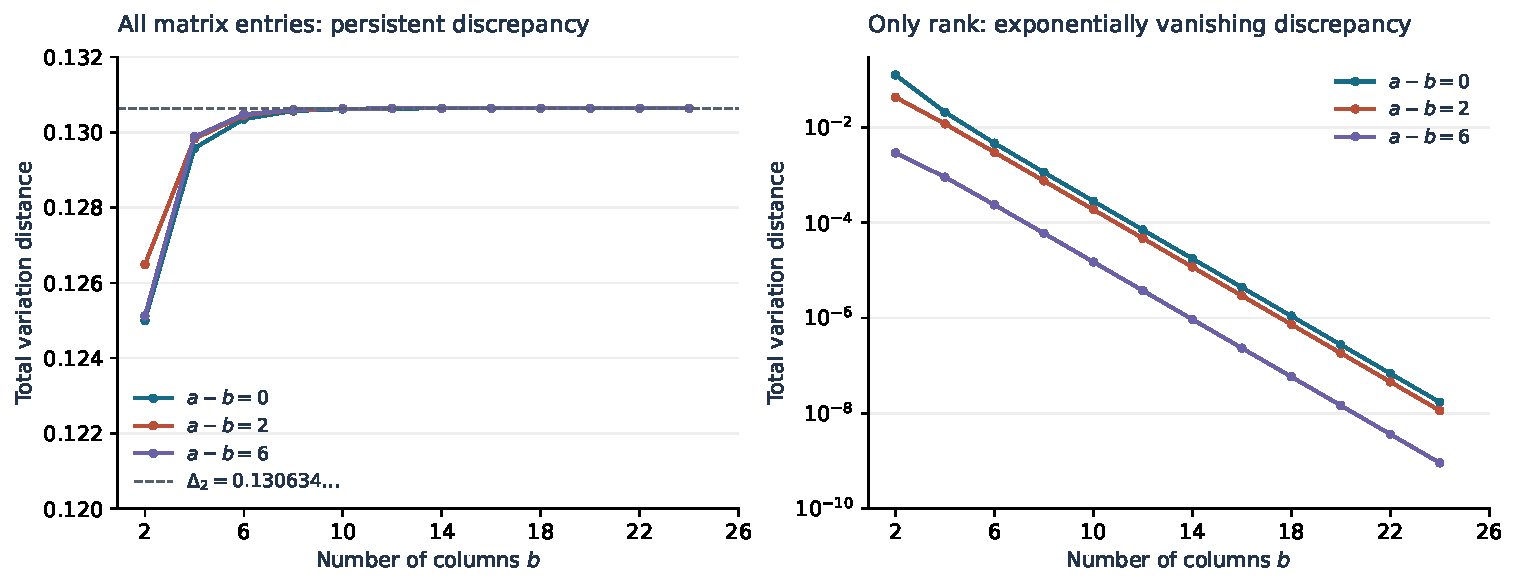
\includegraphics[width=\linewidth]{figures/rank_and_matrix_distance.pdf}
\caption{Exact finite distances over \(\mathbb F_2\), at three fixed
dimension gaps. The full-matrix distance approaches the same positive
constant; the rank distance decays exponentially. The right panel has a
logarithmic vertical scale. The figure is generated from exact fractions,
converted to floating point only for plotting.}
\label{fig:distances}
\end{figure}

\subsection{Numerical constants and verification boundary}

For a product \(\prod_{i>L}(1-t_i)\), with \(0\le t_i\le1\) and summable
\(t_i\), the elementary inequalities
\[
 1-\sum_{i>L}t_i\ \le\ \prod_{i>L}(1-t_i)\ \le\ 1
\]
give rational enclosures of each infinite product.
The supplied \path{results/constant_enclosures.json} uses 64 factors
of \(\eta\) and \(\theta\), and 128 factors of \(\gamma\), to enclose
\(\Delta_q\) for \(q=2,3,4,5\).
All printed digits of \(\Delta_2\) agree at both ends of its enclosure.
The decimal distances in the tables are rounded from exact finite
rational values; no Monte Carlo sampling is used.

The new theorems are proved in ordinary mathematical form.
They have not been formalized or checked by Lean, and inspecting the
repository's upstream formal development does not change that status.
The accompanying formalization plan separates the finite counting,
interpolation, infinite-product, and uniformity obligations.

The principal contribution is the uniform signed comparison and the
centered joint theorem. The full-distance formula is included because
it exhibits the contrast between complete data and rank statistics,
and because a published complement count independently checks it.
The fixed-positive-gap regime posed in the inspected article is
resolved for complementary nondegenerate frames. More general radical
patterns, different ambient complement dimensions, and local-ring
analogues are not treated here.

